\documentclass[10pt, aspectratio=169]{beamer}

\usepackage[utf8]{inputenc}
\usepackage[T1]{fontenc}
\usepackage[ngerman,shorthands=off]{babel}
\usepackage{graphicx}
\usepackage[absolute,overlay]{textpos}
\usetheme{Madrid}
\usecolortheme{seahorse} 
\setbeamertemplate{navigation symbols}{}
\usepackage[backend=biber]{biblatex}
\addbibresource{/Users/jakubmarczak/Downloads/literatur.bib}
\usepackage{csquotes}
\usepackage{hyperref}
\usepackage{wasysym}
\usepackage{xcolor}
\usepackage{tikz}
\definecolor{progress}{HTML}{9b9bba}
\usepackage{listings}
\usepackage{xcolor}
\usetikzlibrary{spy}
\usetikzlibrary{tikzmark,positioning,arrows.meta}
\date{18. Mai 2026}

\lstset{
  language=R,
  basicstyle=\ttfamily\small,
  keywordstyle=\color{blue},
  commentstyle=\color{gray},
  stringstyle=\color{red},
  showstringspaces=false,
  breaklines=true
}

\title[Analyse der Klimaunterschiede in NRW]{Projekt \MakeUppercase{\romannumeral 2}: Analyse der zeitlichen und räumlichen Klimaunterschiede in NRW}
\author[J. Marczak, G. Kathiravan]{Jakub Marczak, Ganeisraaj Kathiravan}

\setbeamertemplate{footline}{
  \leavevmode
  
  % Infoleiste
  \hbox{
    \begin{beamercolorbox}[wd=.333333\paperwidth,ht=2.5ex,dp=1ex,left]{author in head/foot}
      \hspace{1em}\insertshortauthor
    \end{beamercolorbox}
    \begin{beamercolorbox}[wd=.333333\paperwidth,ht=2.5ex,dp=1ex,center]{title in head/foot}
      \insertshorttitle
    \end{beamercolorbox}
    \begin{beamercolorbox}[wd=.333333\paperwidth,ht=2.5ex,dp=1ex,right]{date in head/foot}
      \insertframenumber{} / \inserttotalframenumber \hspace{1em}
    \end{beamercolorbox}
  }

  % Progressbar
  \hbox{
    \begin{beamercolorbox}[wd=\paperwidth,ht=1.3ex,dp=0ex,left]{}
      \tikz{
        \fill[gray!15] (0,0) rectangle (\paperwidth,1.3ex);
        \fill[progress] (0,0) rectangle
        ({\paperwidth*\insertframenumber/\inserttotalframenumber},1.3ex);
      }
    \end{beamercolorbox}
  }
}

\begin{document}

% Folie 1
\begin{frame}[plain]
  \titlepage
\end{frame}

% Folie 2
\begin{frame}
    \frametitle{Inhalt}
    \begin{enumerate}
        \item Datensatz 
        \item Datenaufbereitung
        \item Zentrale Ergebnisse
        \begin{itemize}
            \item Zeitliche Analyse
            \item Räumliche Analyse
            \item Adiabatischer Effekt
        \end{itemize}
        \item Zusammenfassung
    \end{enumerate}
\end{frame}

% Folie 3 
\begin{frame}[fragile]{R Code Beispiel}
    \frametitle{Datensatz}
	\begin{columns}
	
	\column{0.5\textwidth}
        \begin{itemize}
            \item 6 Stationen in Städten an der Ruhr
            \item Variablen
            \item[$\rightarrow$] Jahr
            \item[$\rightarrow$] Mitteltemperatur [$^\circ$C]
            \begin{itemize}
                \item[$\rightarrow$] jährlich
                \item[$\rightarrow$] halbjährlich (Sommer, Winter)
                \item[$\rightarrow$] saisonal (Frühling, Sommer, Herbst, Winter)
                \item[$\rightarrow$] monatlich
            \end{itemize}
        \end{itemize}
        
        \column{0.5\textwidth}
        
    \begin{figure}
        \centering
        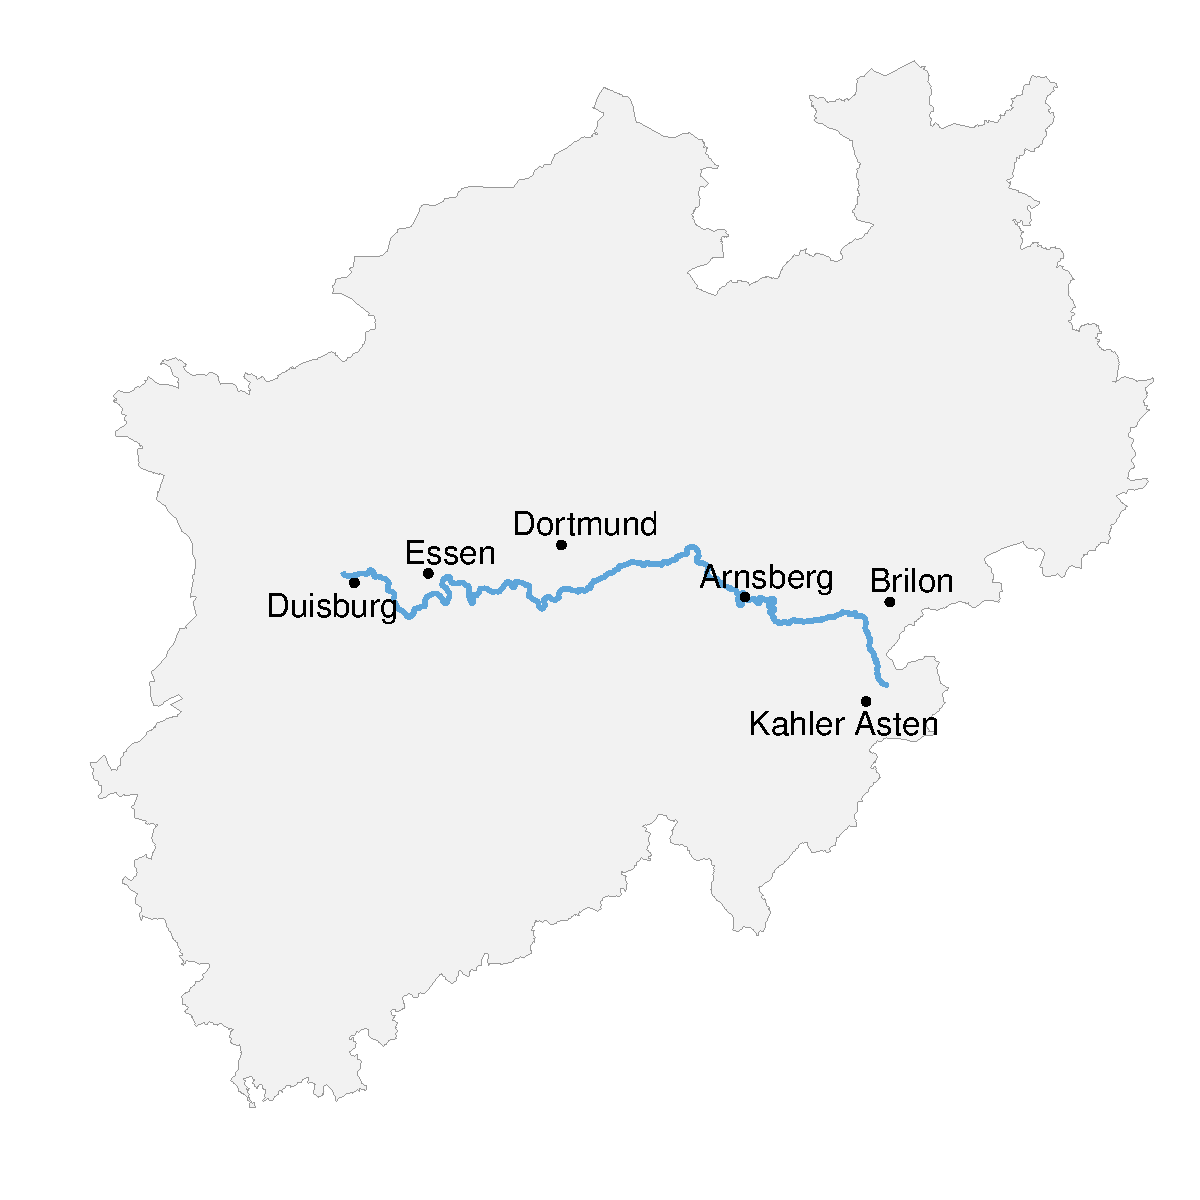
\includegraphics[width=0.9\linewidth]{graphiken/map.pdf}
        \label{fig:map}
    \end{figure}
        \end{columns}
\end{frame}

% Folie 4
\begin{frame}[fragile]{R Code Beispiel}
    \frametitle{Datenaufbereitung}
	\begin{columns}
	
	\column{0.5\textwidth}
        \begin{itemize}
            \item \lstinline{-999999} mit \lstinline{NA} ersetzt
            \item Alle Temperaturen fallen in ein physikalisch plausibles Spektrum für NRW
            \item Es gibt nicht viele und keine stark abweichenden Ausreißer
            \item Bewusstes Ignorieren
        \end{itemize}
        
        \column{0.5\textwidth}
        
    \begin{figure}
        \centering
        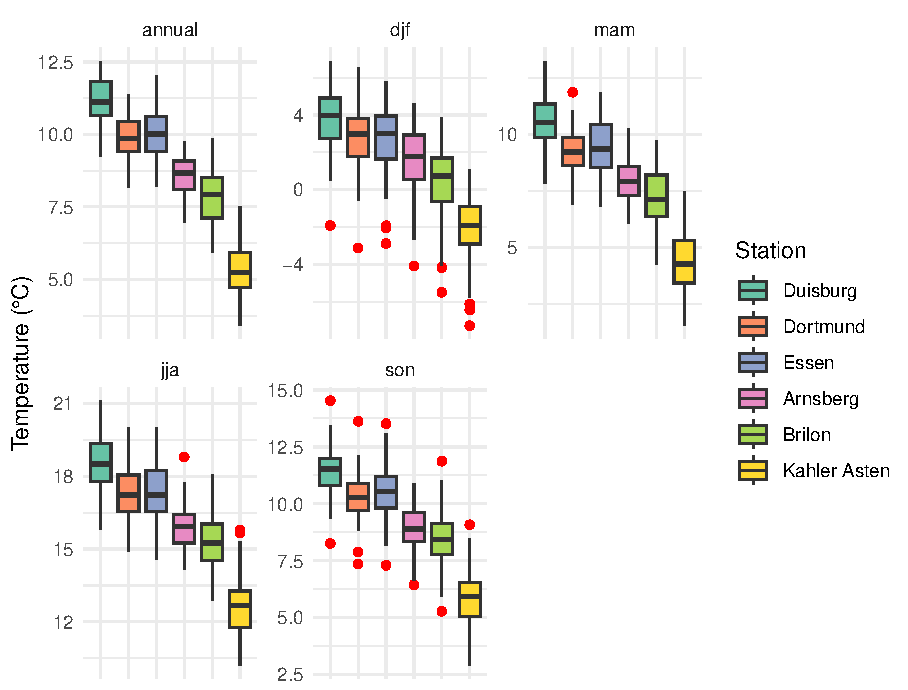
\includegraphics[width=0.95\linewidth]{graphiken/boxplot_outlier_annual_seasonal.pdf}
        \caption{Boxplots der jährlichen und saisonalen Temperaturmittelwerte.}
        \label{fig:boxplotsoutliers}
    \end{figure}
        \end{columns}
\end{frame}

% Folie 5
\section{Zentrale Ergebnisse}

\begin{frame}[plain]
  \centering
  \Huge Zentrale Ergebnisse
\end{frame}

% Folie 6
\begin{frame}[fragile]{R Code Beispiel}
    \frametitle{Zeitliche Analyse}
    \begin{columns}
    
    \column{0.5\textwidth}
    \begin{itemize}
        \item Gewählte Station: Essen
        \begin{itemize}
            \item[i.] 1950 - 1980
            \item[ii.] 1990 - 2020
        \end{itemize}
        \item[$\rightarrow$] Gewählter Test: Welch t-Test
                \begin{itemize}
            \item[$\rightarrow$] H$_0$: $\mu_1 \geq \mu_2$
            \item[$\rightarrow$] H$_1$: $\mu_1 < \mu_2$
            \item $\mu_1$: Mittlere Temp. erster Zeitraum
            \item $\mu_2$: Mittlere Temp. zweiter Zeitraum
        \end{itemize}
        \vspace{-0.22cm}
        \item[$\ast$] {\scriptsize Vorangegangener F-Test}
        \item p-Wert = 3.451e-08 ***
        \item[$\Rightarrow$] Hinweis auf Temperaturerhöhung
        \item Mittelwertdifferenz $\approx$ 1.06 [$^\circ$C]
    \end{itemize}

    
    \column{0.5\textwidth}
    \begin{figure}
        \centering
        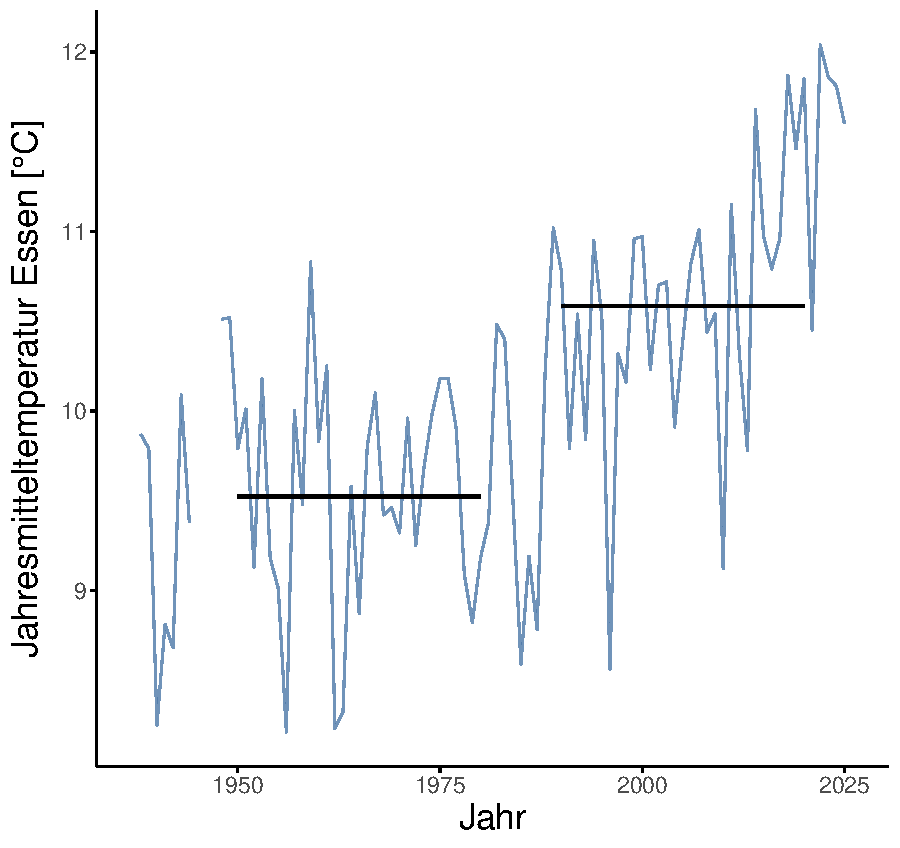
\includegraphics[width=0.8\linewidth]{graphiken/essenjmt.pdf}
        \caption{Zeitreihe von Klimaunterschieden Essens mit Durchschnitten.}
        \label{fig:zeitreiheessen}
    \end{figure}
    \end{columns}
\end{frame}

% Folie 7
\begin{frame}[fragile]{R Code Beispiel}
    \frametitle{Räumliche Analyse}
    
    \begin{columns}

    \column{0.4\textwidth}
        \begin{itemize}
           \item Zeitraum: 1950 - 1995
           \item[$\forall$] Stationen: Beobachtungen relativ vollständig
        	   \item Gruppenvergleich mittels ANOVA- und Tukey-Test
	   \begin{itemize}
        	       \item Normalitätsannahme annähernd erfüllt
            \end{itemize}
            
        \end{itemize}

    \column{0.6\textwidth}
     \only<1>{
        \begin{figure}
        \centering
        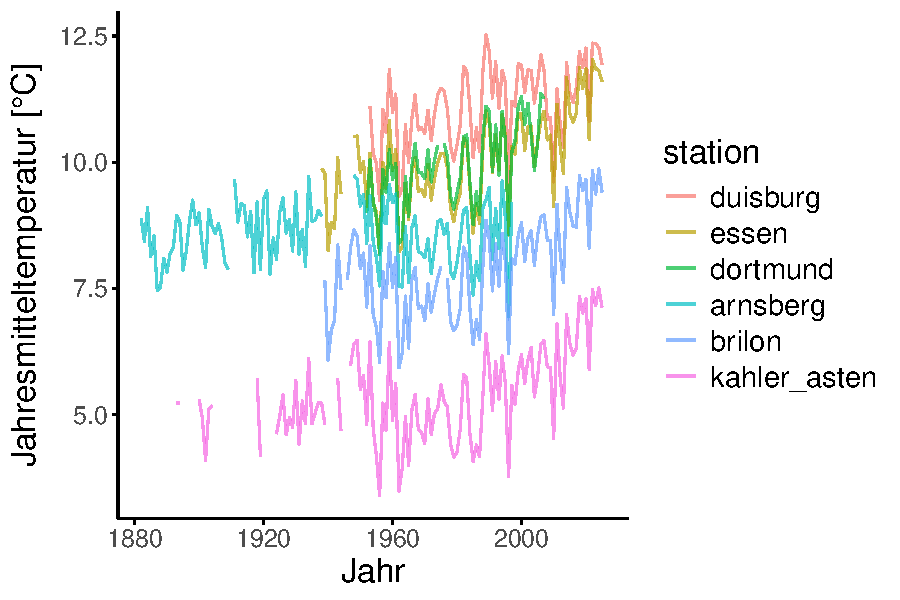
\includegraphics[width=0.9\linewidth]{graphiken/zeitreihe.pdf}
        \caption{Zeitreihen von Temperaturen der Klimastationen.}
        \label{fig:zeitreihen}
     \end{figure}
     }
     
     \only<2>{
        \frametitle{ANOVA-Test}
        \begin{itemize}
           \item \texttt{annual $\sim$ station}
           \item[$\rightarrow$] p-Wert < 2.2e-16 ***
        	   \item[$\Rightarrow$] mindestens zwei Gruppen unterscheiden sich
        \end{itemize}
     }
     
     \only<3>{
        \frametitle{Tukey-HSD-Test}
        \begin{itemize}
           \item Welche Gruppen unterscheiden sich signifikant voneinander?
           \item[$\rightarrow$] Tukey-HSD-Test prüft einzelne Gruppenpaare
        	   \item[$\Rightarrow$] fast alle Gruppen p $\approx$ 0: hochsignifikanter Klimaunterschied
	   \item[$\Rightarrow$] Dortmund - Essen kein signifikanter Unterschied, \newline p = 0.99
        \end{itemize}
     }
     
    \end{columns}
\end{frame}

% Folie 8
\begin{frame}[fragile]{Adiabatischer Effekt}

\only<1>{
\begin{columns}

\column{0.5\textwidth}

\begin{block}{Regressionsmodelle}
\begin{itemize}
   \item Modell 1: \texttt{annual $\sim$ elevation}
   \item[$\rightarrow$] p-Wert $< 2.2\mathrm{e}{-16}$ ***
   \item[$\rightarrow$] $y = 10.78 - 0.0065x_1$
   \item Modell 2: \texttt{annual $\sim$ elevation + station}
   \item[$\rightarrow$] p-Wert $< 2.2\mathrm{e}{-16}$ ***
   \item[$\rightarrow$] $y = 11.35 - 0.0071x_1 - 0.5525x_2 - 1.206x_3$
   \item[$\ast$] $\beta_1$: Höhe, $\beta_2$: Dortmund, $\beta_3$: Arnsberg
\end{itemize}
\end{block}
\vspace{-0.15cm}
{\tiny
$\ast$ Es wurden ausschließlich hochsignifikante Koeffizienten dargestellt.
}

\column{0.5\textwidth}

\begin{itemize}
    \item Adiabatischer Effekt erklärt räumliche Klimaunterschiede wesentlich
    \item[$\rightarrow$] ziemlich genau $-0.65\,^\circ\mathrm{C}/100\,\mathrm{m}$
    \item ANOVA-Test zum Vergleich beider Modelle
    \item[$\rightarrow$] Modell 2 erklärt mehr Varianz als Modell 1
\end{itemize}

\end{columns}
}

     \only<2>{
        \begin{figure}
            \centering
            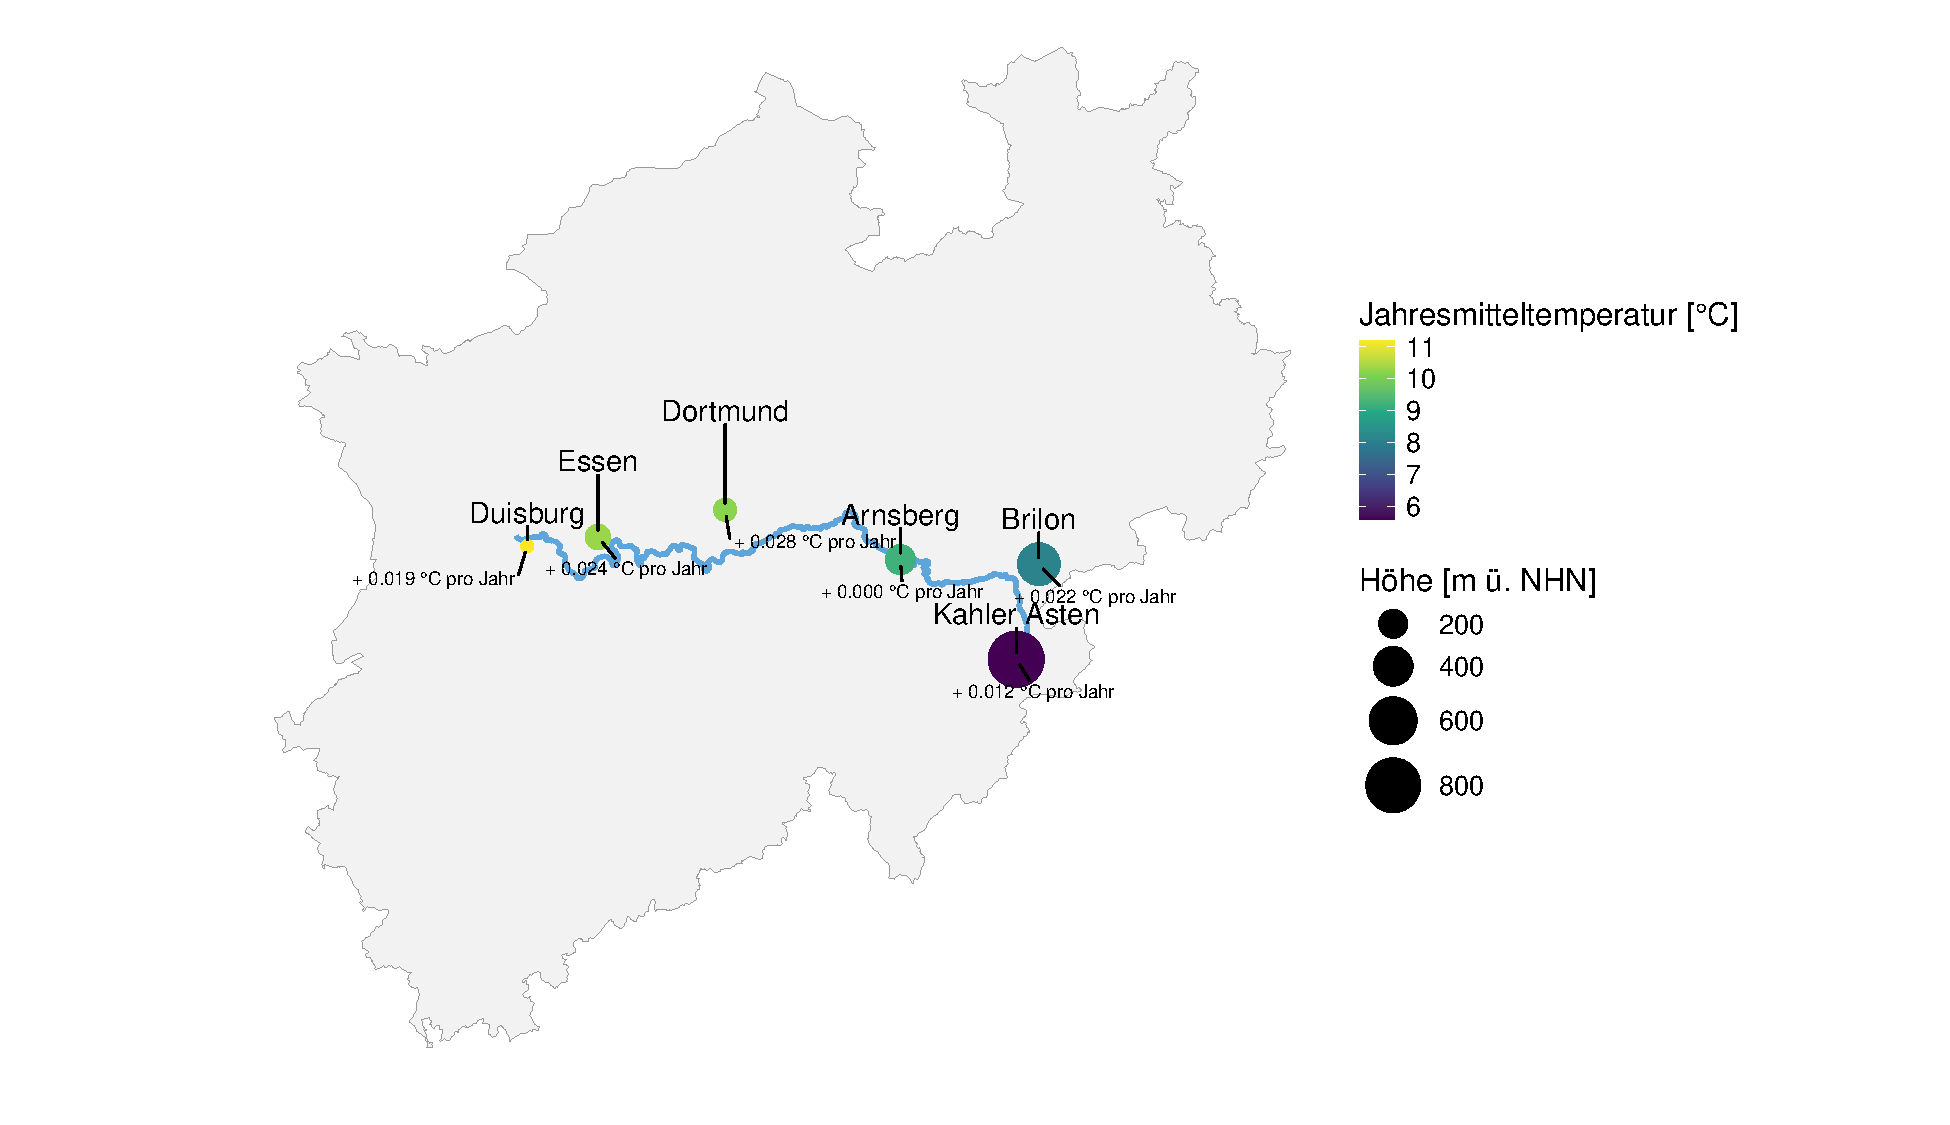
\includegraphics[width=0.7\linewidth]{graphiken/mapdet.pdf}
            \caption{Landkarte des adiabatischen Effekts.}
            \label{fig:mapdet}
         \end{figure}

     }
     
\end{frame}

% Folie 9
\begin{frame}[fragile]{R Code Beispiel}
    \frametitle{Zusammenfassung}
	\begin{itemize}
	    \item Temperaturdaten zeigen zeitliche und räumliche Unterschiede
	    \item Signifikanter Temperaturanstieg in Essen zwischen 1950 - 1980 und 1990 - 2020
	    \item ANOVA zeigt hochsignifikante Unterschiede zwischen den Stationen
	    \item Tukey-HSD-Test: fast alle Stationenpaare unterscheiden sich signifikant
	    \item[$\rightarrow$] Ausnahme: Dortmund - Essen
	    \item Höhenlage erklärt wesentliche räumliche Klimaunterschiede 
	    \item[$\rightarrow$] Temperaturgradient von ca. $-0.65\,^\circ\mathrm{C}/100\,\mathrm{m}$
	    \item[$\Rightarrow$] Zusätzliche standortspezifische Faktoren bleiben relevant
	\end{itemize}

\end{frame}

\end{document}
